\section{Experimental Results}
\begin{table*}[!ht]
\caption{Performance comparison to baselines on classification and regression tasks. The best results are \textbf{bolded} and the second best results are \underline{underlined}. Standard deviations are provided in Sec.~\ref{sec:detailed_experimental_results}.}
\centering
\resizebox{.9\linewidth}{!}{
\begin{tabular}{c}
    % ---------- Table 1 ----------
    \begin{minipage}{\linewidth}
    \centering
    \begin{tabular}{l|cccccc|ccc}
    \hline
    \multirow{3}{*}{Method} & \multicolumn{6}{c|}{UKB} & \multicolumn{3}{c}{ADHD-200} \\ \cline{2-10} 
     & \multicolumn{3}{c|}{Sex} & \multicolumn{3}{c|}{Age} & \multicolumn{3}{c}{Diagnosis} \\
     & ACC & AUC & \multicolumn{1}{c|}{F1} & MSE & MAE & \multicolumn{1}{c|}{$\rho$} &  ACC & AUC & F1 \\ \hline
    XGBoost & 84.1 &0.916&\multicolumn{1}{c|}{0.830} & 0.698 & 0.686 & 0.553 & 62.3 & 0.650 & 0.555 \\
    BrainNetCNN & 91.7 & 0.969 & \multicolumn{1}{c|}{0.912} & 0.597 & 0.618 & 0.647 & 59.2 & 0.640 & 0.545 \\
    BNT & 92.4 & 0.980 & \multicolumn{1}{c|}{0.919} & 0.540 & 0.588 & 0.685 & 63.6 & 0.677 & 0.624 \\
    meanMLP &87.7& 0.949& \multicolumn{1}{c|}{0.919}& 0.672& 0.662& 0.586 & 56.8 & 0.617 & 0.532 \\ 
    Brain-JEPA\footnotemark & 86.8 & 0.943 & \multicolumn{1}{c|}{0.862} & 0.688 & 0.669 & 0.574 & -- & -- & -- \\ \hline
    TFF ($T=20$) & \textbf{98.3} & \underline{0.998} & \multicolumn{1}{c|}{\textbf{0.982}} & 0.440 & 0.525 & 0.760 & 63.3 & 0.700 & 0.608 \\
    SwiFT ($T=20$) & 97.4 &\underline{0.998}& \multicolumn{1}{c|}{0.972}& 0.366 & 0.480 & 0.800 & 63.3 & 0.693 & 0.623 \\
    SwiFT ($T=50$) & \underline{98.1} &\textbf{0.999} &\multicolumn{1}{c|}{\underline{0.980}}& \underline{0.364} & \underline{0.477} & \underline{0.802} & \underline{63.9} & \underline{0.701} & \underline{0.627} \\ \hline
    {\ours} ($T=256$) &97.7& \underline{0.998}& \multicolumn{1}{c|}{0.976} & \textbf{0.340} & \textbf{0.466} & \textbf{0.814} & \textbf{65.8} & \textbf{0.729} & \textbf{0.630}  \\ \hline
    \end{tabular}
    \vspace{0.1in}
    \end{minipage}
    \\[1em] % vertical space
    % ---------- Table 2 ----------
    \begin{minipage}{\linewidth}
    \centering
    \begin{tabular}{l|ccccccccc}
    \hline
    \multirow{3}{*}{Method} & \multicolumn{9}{c}{HCP}  \\ \cline{2-10} 
     & \multicolumn{3}{c|}{Sex} & \multicolumn{3}{c|}{Age} & \multicolumn{3}{c}{Intelligence} \\
     & ACC & AUC & \multicolumn{1}{c|}{F1} & MSE & MAE & \multicolumn{1}{c|}{$\rho$} & MSE & MAE & $\rho$\\ \hline
    XGBoost & 82.2 & 0.890 & \multicolumn{1}{c|}{0.837} & 0.859 & 0.769 & \multicolumn{1}{c|}{0.296} & 0.908 & 0.779 & 0.292 \\
    BrainNetCNN & 86.3 & 0.937 & \multicolumn{1}{c|}{0.866} & 0.847 & 0.749 & \multicolumn{1}{c|}{0.372} & 0.967 & 0.788 & 0.286 \\
    BNT & 86.3 & 0.935 & \multicolumn{1}{c|}{0.872} & 0.794 & 0.719 & \multicolumn{1}{c|}{0.444} & 0.920 & 0.778 & 0.318 \\
    meanMLP & 84.5 & 0.915 & \multicolumn{1}{c|}{0.855} & 0.846 & 0.751 & \multicolumn{1}{c|}{0.370} & 0.887 &0.767  &0.340   \\ 
    Brain-JEPA & 73.9 & 0.809 & \multicolumn{1}{c|}{0.761} & 0.814 & 0.746 & \multicolumn{1}{c|}{0.369} & 0.959 & 0.799 & 0.171\\ 
    \hline
    TFF ($T=20$) & 88.1 & 0.937 & \multicolumn{1}{c|}{0.892} & 0.888 & 0.779 & \multicolumn{1}{c|}{0.246} & 0.898 & 0.767 & 0.312 \\
    SwiFT ($T=20$) & \underline{93.1} & \underline{0.978} & \multicolumn{1}{c|}{\underline{0.937}} & 0.776 & 0.719 & \multicolumn{1}{c|}{0.450} & 0.940 & 0.782 & 0.297  \\
    SwiFT ($T=50$) & 92.2 & 0.972 & \multicolumn{1}{c|}{0.929} & \textbf{0.764} & \textbf{0.699} & \multicolumn{1}{c|}{\underline{0.460}} & \underline{0.865} & \underline{0.758} & \underline{0.354}  \\ \hline
    {\ours} ($T=256$) & \textbf{93.8} & \textbf{0.987} & \multicolumn{1}{c|}{\textbf{0.943}} & \underline{0.773}  & \underline{0.705} & \multicolumn{1}{c|}{\textbf{0.473}} & \textbf{0.835} & \textbf{0.741} & \textbf{0.392}  \\ \hline
    \end{tabular}
    \end{minipage}
\end{tabular}
}
\label{tab:main_results}
\end{table*}

% Please add the following required packages to your document preamble:
% \usepackage{multirow}
\begin{table*}[ht]
\caption{Performance comparison between {\ours} trained from scratch (TFS) and fine-tuned after masked pre-training (FT) on HCP. 
}

\centering
\resizebox{.8\linewidth}{!}{
% \begin{adjustbox}{width=.5\textwidth,center}
\centerline{

\begin{tabular}{l|ccccccccc}
\hline
\multirow{3}{*}{Model} & \multicolumn{9}{c}{HCP}  \\ \cline{2-10} 
 & \multicolumn{3}{c|}{Sex} & \multicolumn{3}{c|}{Age} & \multicolumn{3}{c}{Intelligence}  \\
 & ACC & AUC & \multicolumn{1}{c|}{F1} & MSE & MAE & \multicolumn{1}{c|}{$\rho$} & MSE & MAE & $\rho$ \\ \hline

{\ours} TFS & \meanstd{93.8}{0.9} & \meanstd{\textbf{0.987}}{0.003} & \multicolumn{1}{c|}{\meanstd{0.943}{0.008}} & \meanstd{0.773}{0.077} & \meanstd{\underline{0.705}}{0.038} & \multicolumn{1}{c|}{\meanstd{\underline{0.473}}{0.053}} & \meanstd{\underline{0.835}}{0.053} & \meanstd{\underline{0.741}}{0.028} & \meanstd{\underline{0.392}}{0.062} \\

{\ours} FT & \meanstd{\textbf{95.3}}{1.3} & \meanstd{\underline{0.986}}{0.005} & \multicolumn{1}{c|}{\meanstd{\textbf{0.958}}{0.011}} & \meanstd{\textbf{0.650}}{0.045} & \meanstd{\textbf{0.655}}{0.024} & \multicolumn{1}{c|}{\meanstd{\textbf{0.552}}{0.032}} & \meanstd{\textbf{0.796}}{0.051} & \meanstd{\textbf{0.732}}{0.028} & \meanstd{\textbf{0.435}}{0.046} \\ \hline


\end{tabular}
}% \end{adjustbox}
}


\label{tab:pretraining_results}
\vspace{-3mm}
\end{table*}





\label{sec:experimental results}

\subsection{Experimental Setting}
\label{sec:4.1}
\noindent \textbf{Datasets.}
We used resting-state fMRI data from 8,178 middle-aged and older adults from UK-Biobank (UKB) \citep{UKB}, from 1,061 healthy young adults in the Human Connectome Project (HCP) \citep{HCP}, and from 533 children and adolescents, including both individuals diagnosed with ADHD and healthy controls, included in ADHD-200 \citep{ADHD}.

For UKB and HCP, we used the preprocessed data provided by UK-Biobank \citep{UKB_preproc1, UKB_preproc2} and  HCP \citep{HCP}, which go through the preprocessing pipeline including bias field reduction, skull-stripping, cross-modality registration, and spatial normalization to the MNI space \citep{MNI152}.
For ADHD-200, we used the fMRIPrep \citep{fmriprep1, fmriprep2} processed data from \citet{ADHD} and regressed out nuisance variables using cosine bases, six motion parameters, and aCompCor components.
Following \citet{swift}, we set each fMRI volume to the shape of $(96,96,96)$ by cropping out the background and padding appropriately, and we then applied global min-max normalization and rescaled it to the [$-$1, 1] range to match the input range of the DCAE.

We split UKB and HCP using stratified sampling: by age and sex for UKB, and by age, sex, and intelligence score for HCP.
For the ADHD-200 dataset, we performed stratified sampling based on diagnosis labels and image acquisition sites, following \citet{BNT}.
We generated four different random stratified splits, and for all of the splits, the training, validation, and test sets were assigned in a $0.7:0.15:0.15$ ratio. For the ADHD-200 dataset, we experimented with three random training seeds for each split to ensure reliable results, given the relatively small size of the dataset.

\noindent \textbf{Prediction Targets and Evaluation Metrics.}
We considered sex and age for both UKB and HCP, intelligence (\texttt{CogTotalComp-AgeAdj}) for HCP, and diagnosis for ADHD-200. The continuous targets (age, intelligence) are z-normalized using the training set.
Classification tasks were evaluated with accuracy, AUC (Area Under ROC Curve), and F1 score. Regression tasks were evaluated with MAE (Mean Absolute Error), MSE (Mean Squared Error), and $\rho$ (Pearson’s correlation).

\noindent \textbf{Baselines.}
We considered five ROI-based models as our baseline: XGBoost (eXtreme Gradient Boosting) \citep{xgboost} as a standard machine learning baseline, BrainNetCNN \citep{BNC}, Brain Network Transformer (BNT) \citep{BNT}, meanMLP \citep{meanmlp}, and Brain-JEPA \citep{brainjepa}.
For the Brain-JEPA, we trained a model from scratch for a fair comparison.
To preprocess the data, we first construct the FC matrix using a total of 450 ROIs, comprising 400 ROIs from the Schaefer-400 atlas~\citep{schaefer} and 50 additional ROIs from the Tian-Scale \RNum{3} atlas~\citep{tian}.
For the XGBoost model, we used the upper-triangular FC matrix as the input.
We followed the preprocessing pipeline of Brain-JEPA for its experiments.

For the voxel-based baselines, we adopted TFF \citep{TFF} and SwiFT \citep{swift}, the state-of-the-art voxel-based model. We reproduced the original model with 20 input time frames ($T=20$) for both of them. We also extended SwiFT to our hardware limit ($T=50$) to test possible gains from a longer temporal context; alongside the input time frames, the temporal window size was also extended from $4$ to $10$.



\footnotetext{Since the ADHD-200 dataset contains fMRI data with varying repetition time (TR) values and fewer than 160 frames, the default frame number used in Brain-JEPA, we were unable to conduct experiments.}

\subsection{Main Results}
\label{sec:main_results}
Tab.~\ref{tab:main_results} presents experimental results comparing the performance of different models on a training-from-scratch setting, and the standard deviations are detailed in Sec.~\ref{sec:detailed_experimental_results}. 
We also compare the performance between SwiFT and {\ours} while matching $T$ in \cref{sec:matchted_t} to compare the two models in detail.

The results demonstrate that {\ours} outperforms baseline methods, including both ROI-based and voxel-based approaches, across four tasks and three datasets, with only marginal gains on the HCP-Age task and competitive performance % against voxel-based baselines 
on the UKB-Sex task.

Interestingly, the results of SwiFT ($T=20,50$) and {\ours} indicate a positive association between the number of input time frames ($T$) and performance, in intelligence prediction and ADHD diagnosis, suggesting that modeling longer temporal variability may be particularly advantageous for these tasks. Sec.~\ref{sec:ablation_studies} expands on this observation with a more detailed study.

Although the overall improvement over SwiFT appears modest, we believe this is likely due to two factors: first, the nature of rs-fMRI, in which signals are recorded while subjects are at rest; and second, the tasks considered in our study, which primarily rely on structural information and may not benefit from longer temporal dependencies.

We expect that applying {\ours} to task fMRI data, which contain more temporally dynamic signals, would result in more substantial performance gains over the baselines as it can cover much longer temporal sequences. 
To support this, we provide preliminary experimental results on HBN-Movie \cite{HBN} in \cref{sec:hbn}, where each subject watches two different movies during fMRI acquisition. The results suggest that {\ours} benefits more from extended temporal context compared to the baselines, demonstrating its potential advantage in settings with highly dynamic stimuli.
In addition, investigating a broader range of tasks to determine which ones can benefit from longer temporal information may provide valuable scientific insights. We believe these are promising directions for future work.
% }

\subsection{Effect of Pre-training on Downstream Tasks}
Tab.~\ref{tab:pretraining_results} shows the effectiveness of the masked token pre-training strategy described in Sec.~\ref{sec:masked_pretrain}.
We first pre-trained {\ours} on a large UKB dataset with a 9:1 training and validation split. We then fine-tuned the model on HCP to simulate a transfer learning setting. 
For fine-tuning, we only used 10 epochs, which is considerably fewer compared to training from scratch.
The results demonstrate that the pre-training of {\ours} indeed contributes to the improvement of downstream task performance, albeit with varying amounts of success depending on the task.
\label{sec:pretraining_results}
\begin{table*}[ht]
\caption{Performance comparison between {\ours} with latents from 3D DCAE and 2D DCAE on HCP and ADHD-200. Standard deviations are provided in Sec.~\ref{sec:detailed_experimental_results}.
}
\centering
\resizebox{.8\linewidth}{!}{
\centerline{

\begin{tabular}{l|ccccccccc|ccc}
\hline
\multirow{3}{*}{Tokenizer} & \multicolumn{9}{c|}{HCP} & \multicolumn{3}{c}{ADHD-200} \\ \cline{2-13} 
 & \multicolumn{3}{c|}{Sex} & \multicolumn{3}{c|}{Age} & \multicolumn{3}{c|}{Intelligence} & \multicolumn{3}{c}{Diagnosis} \\
 & ACC & AUC & \multicolumn{1}{c|}{F1} & MSE & MAE & \multicolumn{1}{c|}{$\rho$} & MSE & MAE & $\rho$ & ACC & AUC & F1 \\ \hline

3D DCAE & 92.2 & 0.973 & \multicolumn{1}{c|}{0.929} & \textbf{0.767} & \textbf{0.693} & \multicolumn{1}{c|}{\textbf{0.475}} & 0.869 & 0.755 & \multicolumn{1}{c|}{0.387} & \textbf{65.8} & 0.711 & \textbf{0.644}  \\

2D DCAE & \textbf{93.8} & \textbf{0.987} & \multicolumn{1}{c|}{\textbf{0.943}} & 0.773 & 0.705 & \multicolumn{1}{c|}{0.473} & \textbf{0.835} & \textbf{0.741} & \textbf{0.392} &\textbf{65.8} & \textbf{0.729} & 0.630 \\ \hline



\end{tabular}
}% \end{adjustbox}
}


\label{tab:3D_DCAE_comparison}
\vspace{0mm}
\end{table*}






\subsection{Comparison of 2D Natural Image DCAE and 3D fMRI-trained DCAE}

\label{sec:recon_quality}


To compare the quality of the tokens generated by 2D DCAE and 3D DCAE, we evaluate them in two different aspects: reconstruction quality and downstream performance. The reconstruction quality would serve as a proxy of the crucial information preserved in the latent representations, while the downstream performance would represent the practical impact of the two.

\noindent \textbf{Reconstruction quality.}
We first compare the quality of the fMRI reconstructions from the two autoencoders.
The reconstructions were assessed in two different levels: first, we quantified voxel-level reconstruction fidelity using PSNR, which reflects the preservation of fine-grained intensity details, and SSIM, which captures structural similarity and local spatial patterns. Second, we evaluated the preservation of high-level functional information by comparing the difference in FC matrix between the original fMRI data ($\text{FC}_{\text{orig}}$) and its reconstruction ($\text{FC}_{\text{recon}}$): $||\text{FC}_{\text{orig}}-\text{FC}_{\text{recon}}||_F$.


\begin{figure}
  \centering
  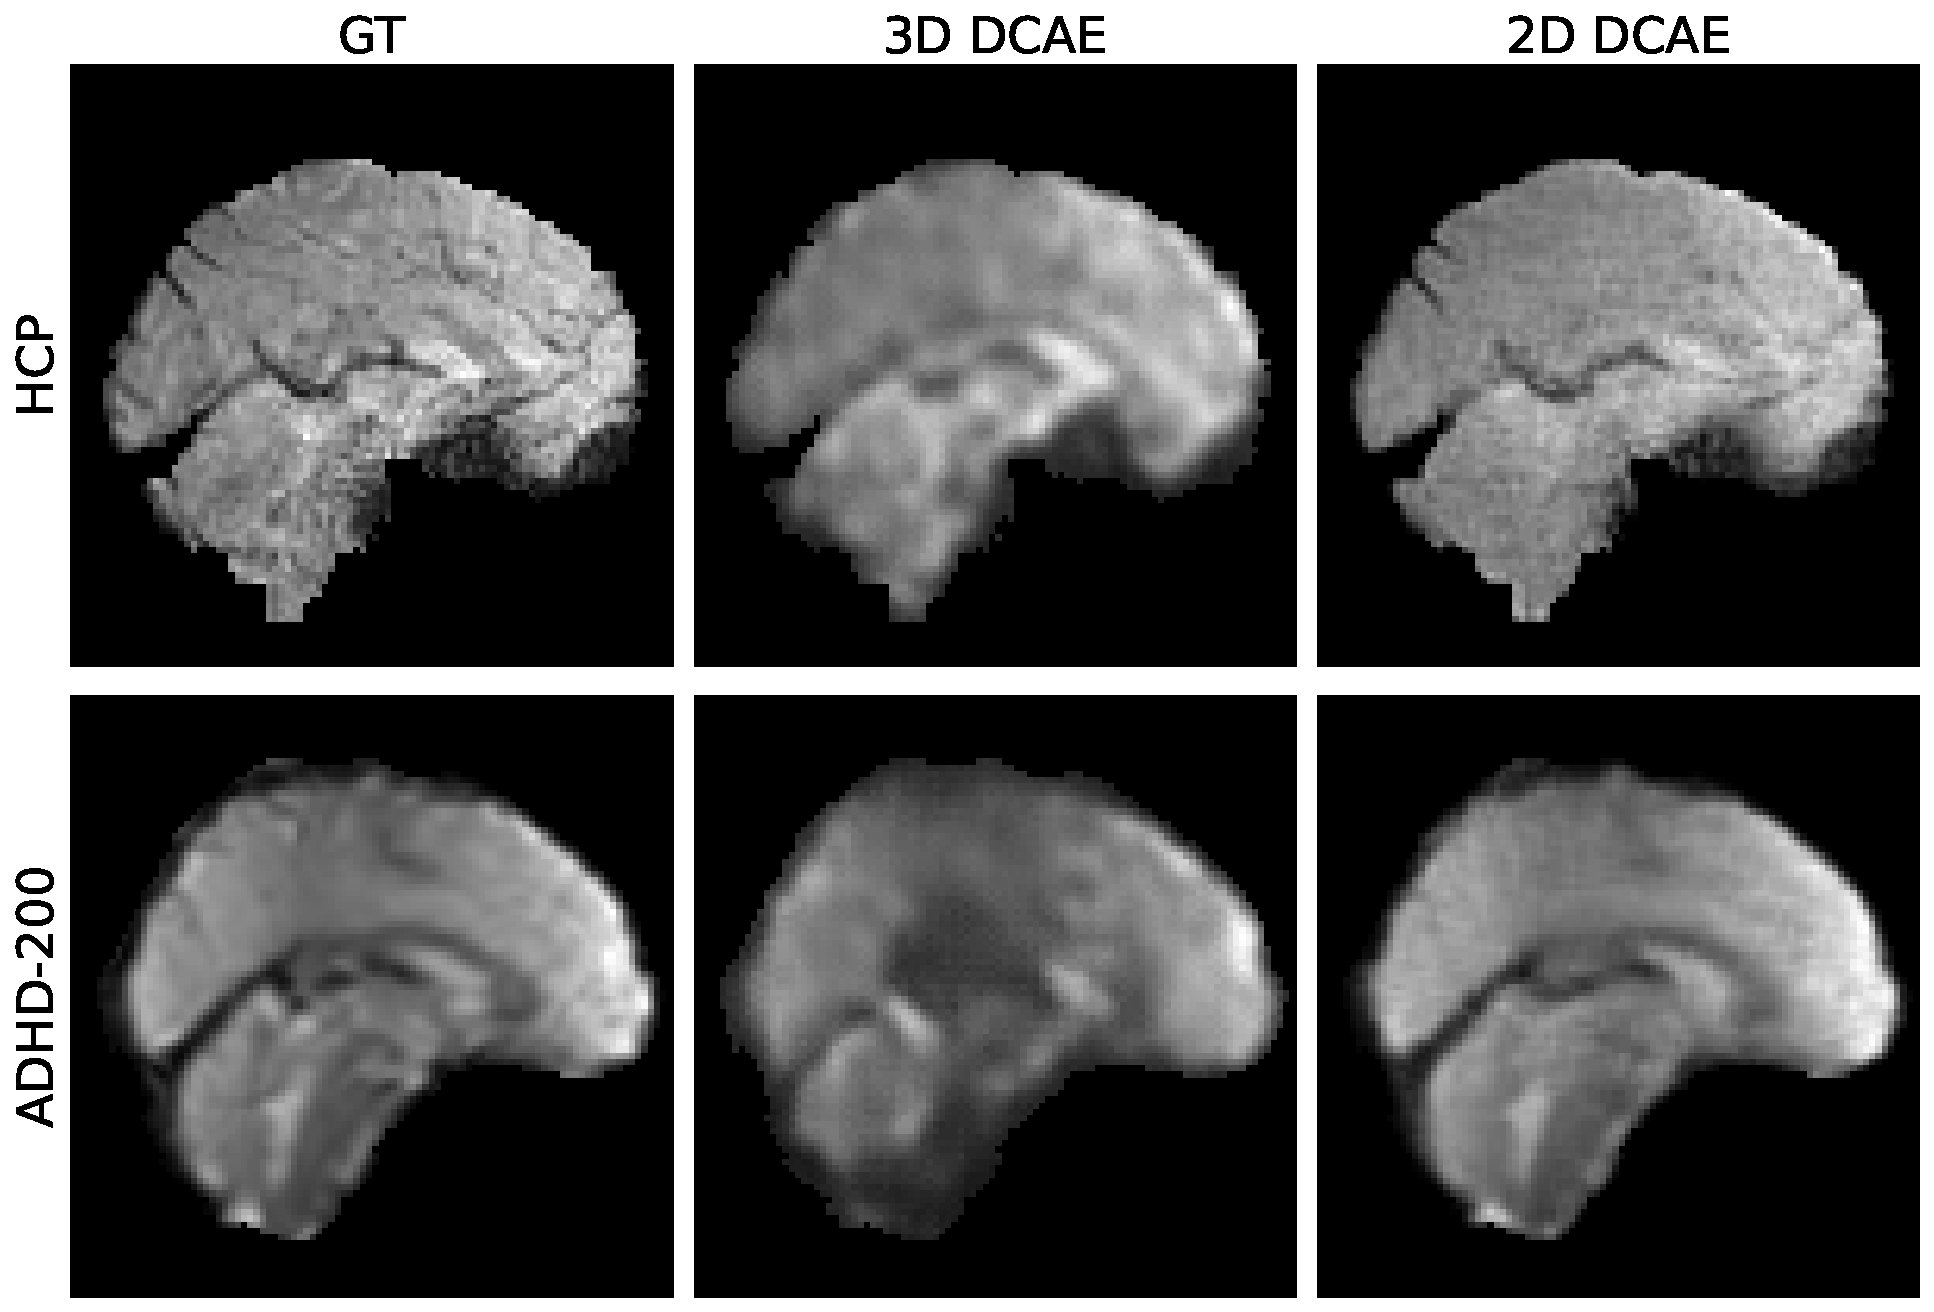
\includegraphics[width=\linewidth]{figures/recon.pdf}
  \caption{Visualization of reconstructions from 3D and 2D DCAE.}
  \label{fig:recon_vis}
  \vspace{-0.1in}
\end{figure}

\begin{figure}
  \centering
  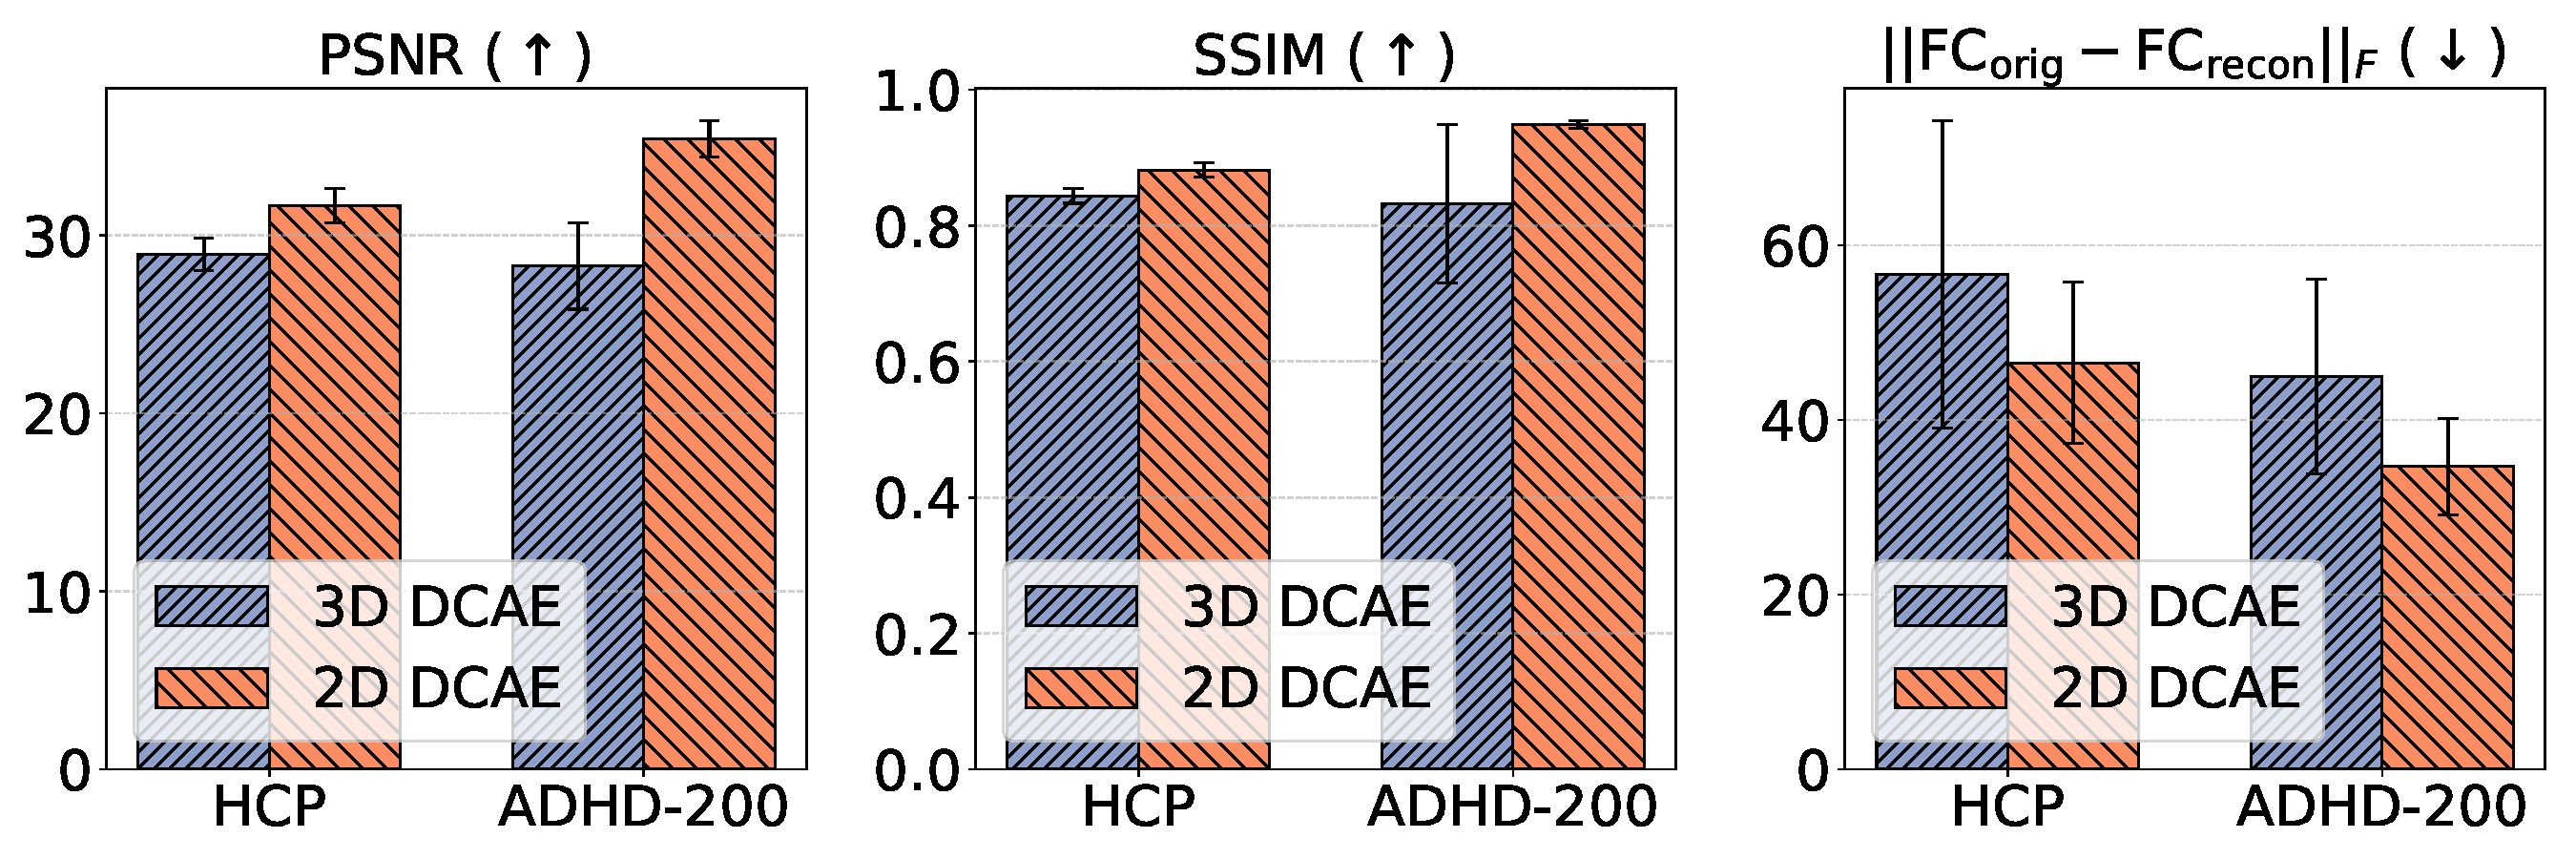
\includegraphics[width=0.9\linewidth]{figures/recon_quality_comparison.pdf}
  \caption{Information preservation of 3D and 2D DCAE.}
  \label{fig:recon_quality}
  \vspace{-5mm}
\end{figure}
\begin{figure*}[ht!]
  \centering
  \begin{subfigure}[t]{0.42\linewidth}
    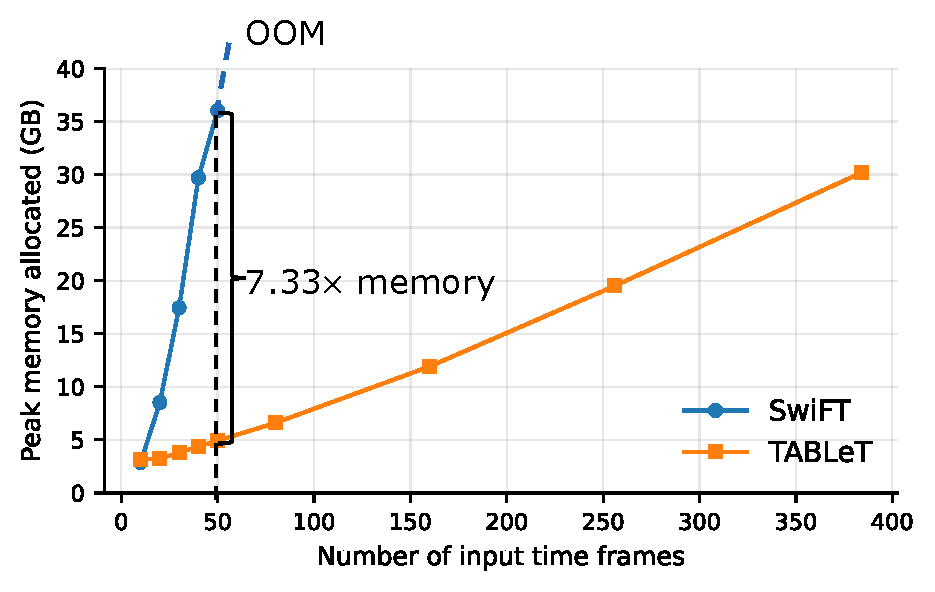
\includegraphics[width=\linewidth]{figures/memory_comparison_fig.pdf}
    \caption{Peak memory allocation}
    \label{fig:left}
  \end{subfigure}
  \begin{subfigure}[t]{0.42\linewidth}
    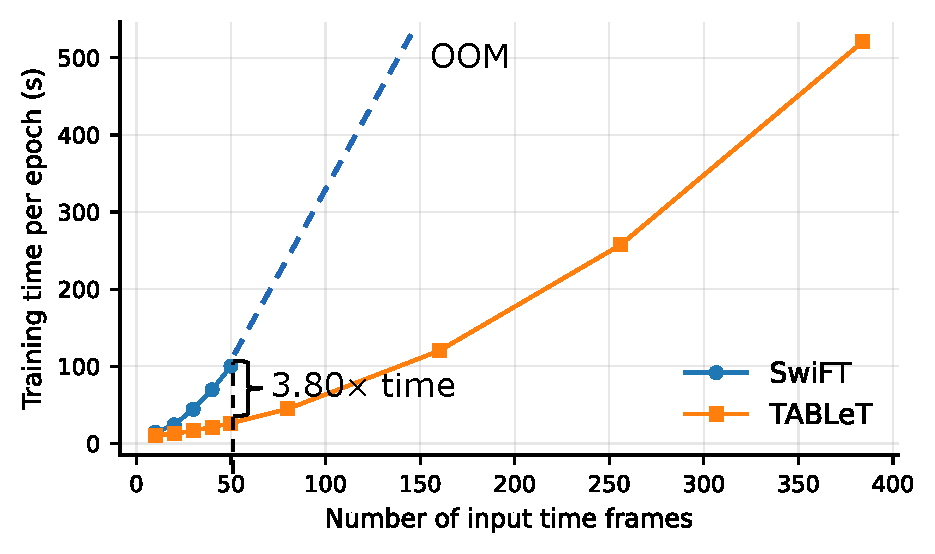
\includegraphics[width=\linewidth]{figures/time_comparison_fig.pdf}
    \caption{Training time per epoch}
    \label{fig:right}
  \end{subfigure}
  \caption{Comparison of (a) memory and (b) training time, between {\ours} and SwiFT.}
  \label{fig:both}
  % \vspace{-3mm}
\end{figure*}
The 3D DCAE was trained with the UKB dataset; a detailed training procedure is provided in Sec.~\ref{sec:training_3D_DCAE}.
To assess generalizability, we deliberately excluded HCP and ADHD-200 from the training set. The reconstructions from the three slicing axes were averaged for 2D DCAE.

The 2D DCAE moderately outperformed the 3D DCAE both qualitatively and quantitatively, as shown in Fig.~\ref{fig:recon_vis} and Fig.~\ref{fig:recon_quality}.
This result suggests that the 2D DCAE, pre-trained on massive, diverse natural image datasets, learns highly robust and general-purpose low-level feature extractors (e.g., for edges, textures), and in turn is able to generalize well into medical images.
Moreover, the 2D DCAE also better preserved functional connectivity patterns, indicating that its latent representations retain high-level functional relationships in the brain.

As a side note, we also attempted to fine-tune the 2D DCAE with fMRI data while freezing different parts of the autoencoder, but discovered that any fine-tuning consistently harmed the reconstruction quality. We presume this is because our fMRI dataset is relatively small and homogeneous compared to the dataset the model is trained on, potentially harming generic filters crucial for the model's generalization capabilities. 

\noindent \textbf{Downstream Performance.}
We also compare {\ours} models trained with latents from the 3D DCAE and the 2D DCAE. The experiment setup is identical to the one detailed in ~\cref{sec:4.1} and ~\cref{sec:main_results}. 
As shown in Tab.~\ref{tab:3D_DCAE_comparison}, both models achieve comparable performance, with the 2D DCAE moderately outperforming the 3D counterpart in most cases.

Overall, these results indicate that a 2D DCAE, despite never being trained on fMRI, generalizes well as a tokenizer for 4D fMRI, both in terms of reconstruction fidelity and downstream performance. Given its strong performance, alongside the practical benefit of avoiding costly dataset collection or additional fine-tuning, we advocate using an existing 2D DCAE as a training-free tokenizer rather than building and training a dedicated 3D counterpart. 



\subsection{Memory and Computational Efficiency}

We conduct a quantitative analysis to compare the memory and computational efficiency between {\ours} and SwiFT. To ensure a fair comparison, all tests were performed on a single NVIDIA RTX A6000 GPU, and the batch size of both models was fixed to 4. 
We were only able to run SwiFT up to $T=50$ due to memory limitations. At $T=50$, compared to SwiFT, {\ours} is 7.33 times more memory efficient, and trains 3.8 times faster. With a similar memory budget ($\sim$30GB), $T$ can be extended nearly tenfold between SwiFT ($T=40$) and {\ours} ($T=384$).





\subsection{Additional Ablation Studies}
\label{sec:ablation_studies}
\noindent \textbf{Effect of Aggregation of Three Axes.}
We examined the effect of axis aggregation to better understand its effect: we compared models trained with fMRI tokens derived from a single axis alongside the model with aggregated tokens.
As shown in Tab. \ref{tab:axis_ablation}, the performance of {\ours} varies depending on the chosen axis for single-axis models.
In contrast, our aggregated version consistently achieves strong performance across tasks, eliminating the dependence on any particular slicing axis. We chose to aggregate all three axes instead of using a single axis due to this reliability.
\begin{table*}[ht]
\centering
\caption{Effect of the choice of slicing axis and aggregation of the three axes on classification and regression tasks. The best results are \textbf{bolded} and the second best results are \underline{underlined}.}
\resizebox{.85\linewidth}{!}{%
\begin{minipage}{\linewidth}
    % ---------- Subtable 1 ----------
    \centering
    \begin{tabular}{l|cccccc}
    \hline
    \multirow{3}{*}{Axis} & \multicolumn{6}{c}{UKB}  \\ \cline{2-7} 
     & \multicolumn{3}{c|}{Sex} & \multicolumn{3}{c}{Age}  \\
     & ACC & AUC & \multicolumn{1}{c|}{F1} & MSE & MAE & \multicolumn{1}{c}{$\rho$}\\ \hline

    Sagittal & \meanstd{\underline{97.3}}{0.9} & \meanstd{0.996}{0.001} & \multicolumn{1}{c|}{\meanstd{\underline{0.971}}{0.009}} & \meanstd{\underline{0.369}}{0.015} & \meanstd{\underline{0.486}}{0.010} & \multicolumn{1}{c}{\meanstd{\underline{0.796}}{0.008}} \\
    Coronal& \meanstd{97.1}{0.4} & \meanstd{0.996}{0.002} & \multicolumn{1}{c|}{\meanstd{0.969}{0.004}} & \meanstd{0.435}{0.012} & \meanstd{0.525}{0.008} & \multicolumn{1}{c}{\meanstd{0.756}{0.009}}   \\
    Axial & \meanstd{\underline{97.3}}{0.4} & \meanstd{\underline{0.997}}{0.000} & \multicolumn{1}{c|}{\meanstd{\underline{0.971}}{0.004}} & \meanstd{0.410}{0.020} & \meanstd{0.509}{0.014} & \multicolumn{1}{c}{\meanstd{0.771}{0.013}}  \\ \hline

    {All}& \meanstd{\textbf{97.7}}{0.2} & \meanstd{\textbf{0.998}}{0.000} & \multicolumn{1}{c|}{\meanstd{\textbf{0.976}}{0.002}} &  \meanstd{\textbf{0.340}}{0.011} & \meanstd{\textbf{0.466}}{0.010} & \multicolumn{1}{c}{\meanstd{\textbf{0.814}}{0.009}} \\ \hline
    \end{tabular}
    
    \vspace{1em} % <-- space between subtables

    % ---------- Subtable 2 ----------
    \centering
    \begin{tabular}{l|cccccc}
    \hline
    \multirow{3}{*}{Axis} & \multicolumn{6}{c}{HCP}  \\ \cline{2-7} 
     & \multicolumn{3}{c|}{Sex} & \multicolumn{3}{c}{Age}  \\
     & ACC & AUC & \multicolumn{1}{c|}{F1} & MSE & MAE & \multicolumn{1}{c}{$\rho$}\\ \hline

    Sagittal & \meanstd{91.3}{3.6} & \meanstd{0.972}{0.017} & \multicolumn{1}{c|}{\meanstd{0.920}{0.033}} & \meanstd{0.783}{0.111} & \meanstd{0.721}{0.041} & \multicolumn{1}{c}{\meanstd{0.458}{0.076}} \\
    Coronal& \meanstd{\underline{93.6}}{1.7} & \meanstd{\underline{0.981}}{0.007} & \multicolumn{1}{c|}{\meanstd{\underline{0.941}}{0.015}} & \meanstd{0.855}{0.053} & \meanstd{0.745}{0.023} & \multicolumn{1}{c}{\meanstd{0.376}{0.048}}   \\
    Axial & \meanstd{92.3}{3.0} & \meanstd{0.979}{0.008} & \multicolumn{1}{c|}{\meanstd{0.930}{0.028}} & \textbf{\meanstd{\textbf{0.748}}{0.056}} & \meanstd{\underline{0.711}}{0.015} & \multicolumn{1}{c}{\meanstd{\underline{0.470}}{0.040}}  \\ \hline

    {All}& \meanstd{\textbf{93.8}}{0.9} & \meanstd{\textbf{0.987}}{0.003} & \multicolumn{1}{c|}{\meanstd{\textbf{0.943}}{0.008}} &  \meanstd{\underline{0.773}}{0.077} & \meanstd{\textbf{0.705}}{0.038} & \multicolumn{1}{c}{\meanstd{\textbf{0.473}}{0.053}} \\ \hline
    \end{tabular}

    \vspace{1em} % <-- space between subtables

    % ---------- Subtable 3 ----------
    \centering
    \begin{tabular}{l|cccccc}
    \hline
    \multirow{3}{*}{Axis} & \multicolumn{3}{c}{HCP} & \multicolumn{3}{c}{ADHD-200}  \\ \cline{2-7} 
     & \multicolumn{3}{c|}{Intelligence} & \multicolumn{3}{c}{Diagnosis}  \\
     & MSE & MAE & \multicolumn{1}{c|}{$\rho$} & ACC & AUC & \multicolumn{1}{c}{F1}\\ \hline

    Sagittal & \meanstd{\underline{0.842}}{0.058} & \meanstd{\underline{0.744}}{0.028} & \multicolumn{1}{c|}{\meanstd{\textbf{0.401}}{0.060}} & \meanstd{\textbf{65.8}}{2.3} & \meanstd{\underline{0.715}}{0.026} & \multicolumn{1}{c}{\meanstd{\textbf{0.633}}{0.032}} \\
    Coronal& \meanstd{0.850}{0.057} & \meanstd{0.749}{0.029} & \multicolumn{1}{c|}{\meanstd{0.381}{0.065}} & \meanstd{63.5}{3.1} & \meanstd{0.707}{0.036} & \multicolumn{1}{c}{\meanstd{0.621}{0.040}}   \\
    Axial & \meanstd{0.896}{0.070} & \meanstd{0.773}{0.033} & \multicolumn{1}{c|}{\meanstd{0.309}{0.072}} & \textbf{\meanstd{\underline{64.3}}{2.5}} & \meanstd{0.713}{0.022} & \multicolumn{1}{c}{\meanstd{0.622}{0.034}}  \\ \hline

    {All}& \meanstd{\textbf{0.835}}{0.053} & \meanstd{\textbf{0.741}}{0.028} & \multicolumn{1}{c|}{\meanstd{\underline{0.392}}{0.062}} &  \meanstd{\textbf{65.8}}{3.5} & \meanstd{\textbf{0.728}}{0.020} & \meanstd{\underline{0.630}}{0.038} \\ \hline
    \end{tabular}
\end{minipage}
}
% \vspace{0.1in}
\label{tab:axis_ablation}
\end{table*}





\noindent \textbf{Effect of $T$.}
\begin{figure}[ht!]
  \centering
  \begin{subfigure}[t]{0.495\linewidth}
    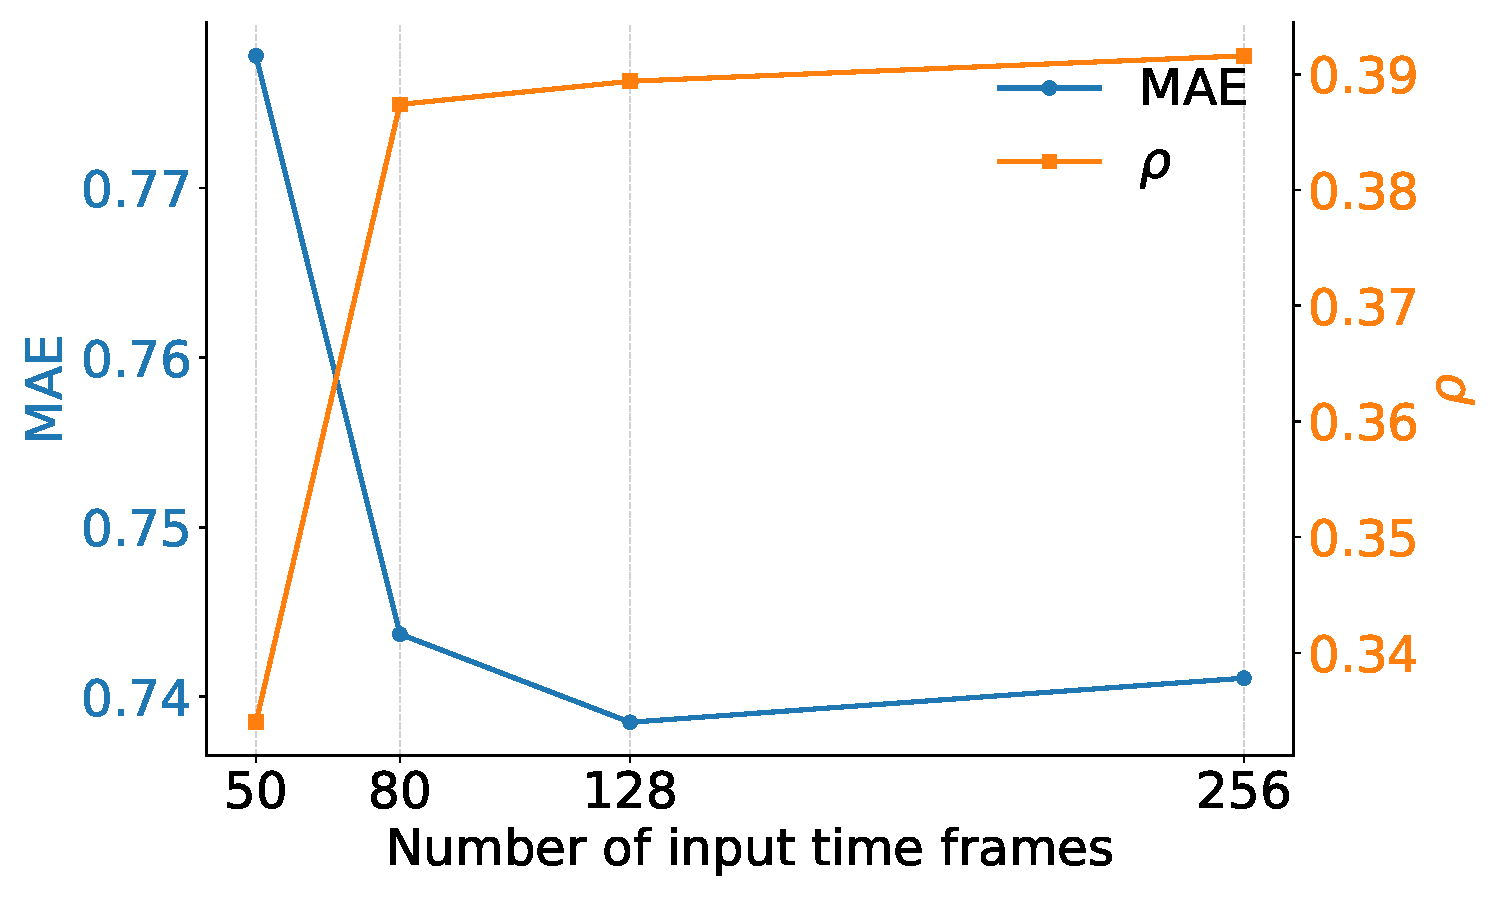
\includegraphics[width=\linewidth]{figures/hcp_time_window_ablation.pdf}
    \caption{HCP-Intelligence}
    \label{fig:t_left}
  \end{subfigure}
  \begin{subfigure}[t]{0.495\linewidth}
    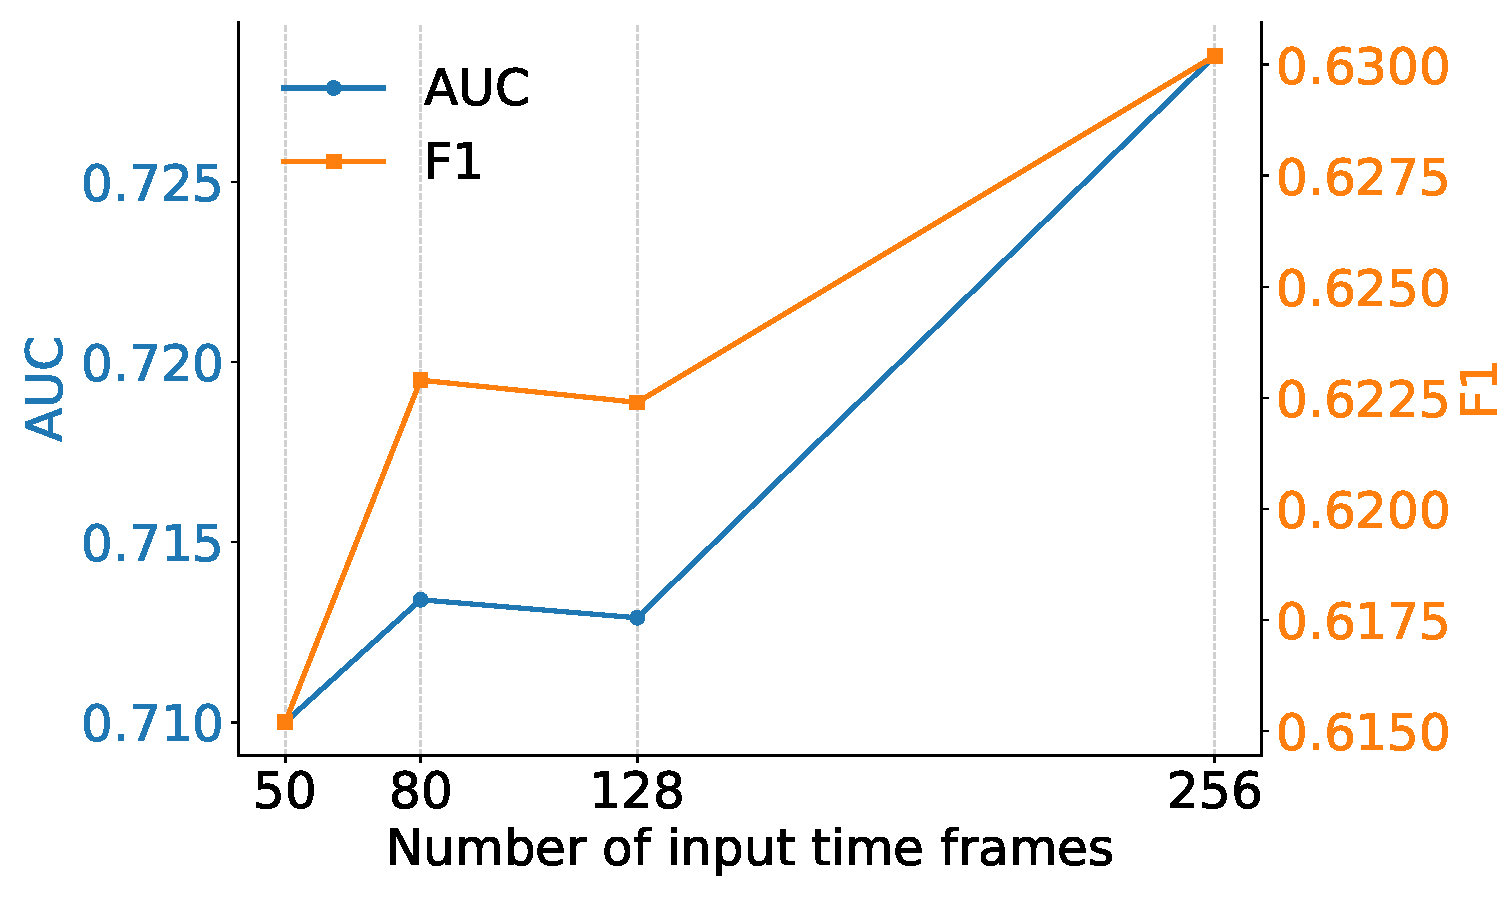
\includegraphics[width=\linewidth]{figures/adhd_time_window_ablation.pdf}
    \caption{ADHD-200}
    \label{fig:t_right}
  \end{subfigure}
  \caption{Performance of {\ours} on HCP-Intelligence and ADHD-200 with varying $T$.}
  \vspace{-3mm}
  \label{fig:t_ablation}
\end{figure}
As shown in Tab.~\ref{tab:main_results}, modeling longer-range temporal dynamics can improve performance on the HCP-Intelligence and ADHD diagnosis tasks. To explore this further, we varied the $T$ of {\ours} and evaluated the corresponding performance. Interestingly, Fig.~\ref{fig:t_ablation} reveals a clear positive trend between performance and $T$. We believe that investigating the relationship between $T$ and model performance across diverse tasks represents a promising direction for future research.

\subsection{Interpretation Results}

One advantage of voxel-based methods is that the models are interpretable, since the entire process from voxel to prediction is differentiable. To test the interpretability of {\ours},
we used Integrated Gradients (IG) \citep{IG} for visualization of highly contributing areas for sex-classification. We used female test subjects in the HCP-Sex task who are correctly classified with {\ours} with high confidence ($\ge75\%)$, and computed the IG map of the first frame from each subject, then averaged it.
\begin{wrapfigure}{r}{0.2\textwidth}
  \vspace{-0.15in}
  \centering
  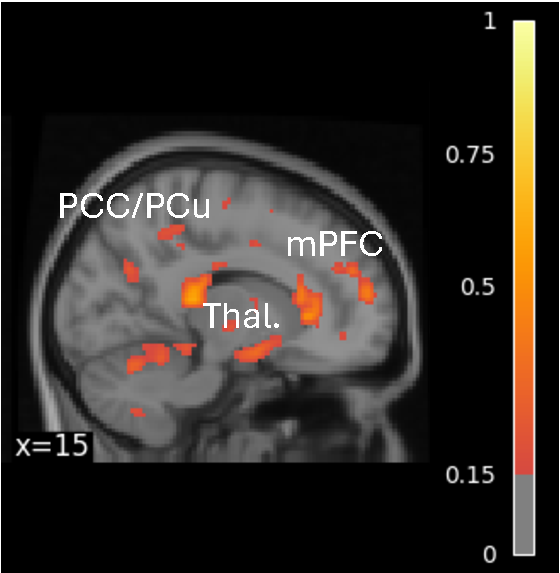
\includegraphics[width=\linewidth]{figures/ig.pdf}
  \caption{IG map.}
  \label{fig:ig}
  \vspace{-0.3in}
\end{wrapfigure}

Fig.~\ref{fig:ig} shows that {\ours} mainly focuses on the medial prefrontal gyrus (mPFC), posterior cingulate cortex (PCC), precuneus (PCu), and thalamus (Thal.), regions commonly implicated in brain sex difference literature \citep{sexdiff1, sexdiff2, sexdiff3, sexdiff4}.
